\documentclass [9 pt]{article}
\usepackage[margin = 1in]{geometry}
\usepackage{amsfonts}
\usepackage{amsthm}
\usepackage{bbm}
 \usepackage{amsmath}
\usepackage[utf8]{inputenc}
\usepackage{graphicx}
\usepackage{enumerate}
\usepackage{color}
\usepackage{graphicx}
\graphicspath{ {./images/} }
\usepackage{tikz}

\theoremstyle{definition}
\newtheorem{problem}{Problem}
\newtheorem{theorem}{Theorem}
\newtheorem*{corollary}{Corollary}
\newtheorem{proposition}[theorem]{Proposition}
\newtheorem{lemma}[theorem]{Lemma}
\newtheorem{conjecture}[theorem]{Conjecture}

\newtheorem{definition}[theorem]{Definition}
\newtheorem{remark}[theorem]{Remark}
\newtheorem{example}[theorem]{Example}


\usepackage{fancyhdr}
\pagestyle{fancy}
\lhead{Yuhao Wu \quad 260711365} 
\rhead{\bfseries COMP 330 Assignment 1}
\cfoot{\thepage}
\renewcommand{\headrulewidth}{0.4pt}
\renewcommand{\footrulewidth}{0.4pt}





\begin{document}

\title{COMP 330 Assignment 1}
\date{2018-9-15}
\author{Name: Yuhao Wu\\
ID Number: 260711365
}
\maketitle


\section*{Question 5:}
(1): Give a deterministic finite automaton accepting the following language over the alphabet $\{0, 1\}$: The set of all words containing 100 or 110. \\
\newline
(2): Show that any $DFA$ for recognizing this language must have at least 5 states. 
\subsection*{(1):}
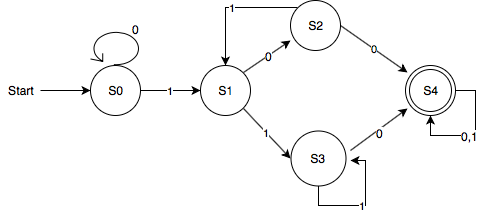
\includegraphics[scale = 0.8]{Q5.png}
\begin{itemize}
	\item $S_0$ means the last three bits are 000
	\item $S_1$ means the last three bits are 001, 101
	\item $S_2$ means the last three bits are 010, when the next is 1, as the automata can't recognize something like 101, so have to go back to $S_1$
	\item $S_3$ means the last three bits are 011, 111, when the next is 1, have to go back to itself
	\item $S_4$ means the word contains 100 or 110, since the automata just wants to recognize words containing 100 or 110, when reading more letters, it stays in $S_4$, which is our accept state.
\end{itemize}
\subsection*{(2):}
\begin{proof}
	As I have already draw a DFA for Question1 using 5 states, what we need to do is to prove that it is impossible for any DFA recognizing this language having only 4 states.\\
	\newline
	As the purpose of the automata is to recognize words containing 100 or 110, which means the automata at least needs to store 3 bits, otherwise how could it be able to recognize 3 bits words.\\
	\newline
	All the possible permutation of 3 bits words is below:
	$$\{000, 001, 010, 011, 100, 101, 110, 111 \}$$
	Obviously, we can separate $\{ 100 , 110 \}$ from above, as they are accept states and others are reject states.\\
	\newline
	Then, we can separate $\{ 010, 011, 111 \}$ from above, as they ends in 11 or 10, when the next bit is 0, they can change into accept states.\\
	But, in fact, we have to separate the three elements, as when the following bits is 1, 010 will change into 101, which is not in this sets.\\
	\newline
	Under this case, we have already had four states:
	\begin{itemize}
		\item $\{100, 110\} \implies$ accepting states
		\item $\{011, 111 \} \implies$ after adding 1, it will still be in this state, after adding 0, it will go to accepting states
		\item  $\{010 \} \implies$ after adding 1, it will go to the fourth state, after adding 0, it will go to accepting states
		\item  $\{ 000, 001, 101 \} $ this is the remaining 
	\end{itemize} 
	For the fourth state, when the next coming bit is 0, 000 will stay in the same states, while 001 and 101 will go to the third state,  and get a contradiction. \\
	So, we can conclude that any $DFA$ for recognizing this language must have at least 5 states. \\
\end{proof}



\end{document}